\documentclass[a4paper]{article}

\usepackage[a4paper,  margin=1.0in]{geometry}

\usepackage{graphicx}
\usepackage{float}
\usepackage{hyperref}
\usepackage{pgfplots}




\usepackage{polski}
\usepackage[utf8]{inputenc}

\begin{document}


\title{ Laboratorium Rozpoznawania Obrazów – Ćwiczenie \#5 \& \#6 Rozpoznawanie cyfr z wykorzystaniem sieci neuronowych}

% crann.m - init
% TODO- actf, backprop, actdf (pochodna aktywacji)
% bez mini matchów (patrz pętla w backprop.m)


\author{Michał Sypetkowski}
\maketitle


\section{Ogólne uwagi}
Eksperymenty przeprowadzane są na zbiorze danych MNIST
\footnote{\url{http://yann.lecun.com/exdb/mnist/}}
Mamy 60k przykładów trenujących i 10k do testowania.
Zbiór trenujący - pliki:
\begin{verbatim}
train-images-idx3-ubyte
train-labels-idx1-ubyte
\end{verbatim}

Zbiór testujący:
\begin{verbatim}
t10k-images-idx3-ubyte
t10k-labels-idx1-ubyte
\end{verbatim}

W pliku \texttt{ann\_training.m} ustawiane jest ziarno losowe (123) dla powtarzalności eksperymentów.

\section{Model podstawowy}

Uczymy perceptron 2 warstwowy przez 6 epok.
Wielkość warstwy ukrytej to 200.
Współczynnik uczenia to 0.005 przez cały czas uczenia.
Funkcja straty to MSE (Mean Squared Error) a funkcja aktywacji -- relu.

Precyzja na zbiorze testującym po kolejnych epokach (końcowo około 0.974):

% \begin{figure}[H]
%     \caption{Błąd na zbiorze testującym po kolejnych epokach
%     \label{fig:graph}
%     }
\begin{center}
\begin{tikzpicture}
\begin{axis}
    \addplot[color=red,mark=x] coordinates {
        (1.000000 ,  1- 0.045800)
        (2.000000 ,  1- 0.034200)
        (3.000000 ,  1- 0.030600)
        (4.000000 ,  1- 0.029600)
        (5.000000 ,  1- 0.026900)
        (6.000000 ,  1- 0.025700)
    };
\end{axis}
\end{tikzpicture}
\end{center}
% \end{figure}

\section{Opadający współczynnik uczenia}

Wprowadziłem wykładnicze opadanie współczynnika uczenia.
Precyzja na zbiorze testującym po kolejnych epokach
(pomarańczowy - zmniejszanie współczynnika 0.5 raza z każdą epoką,
zielony - 0.75):
\begin{center}
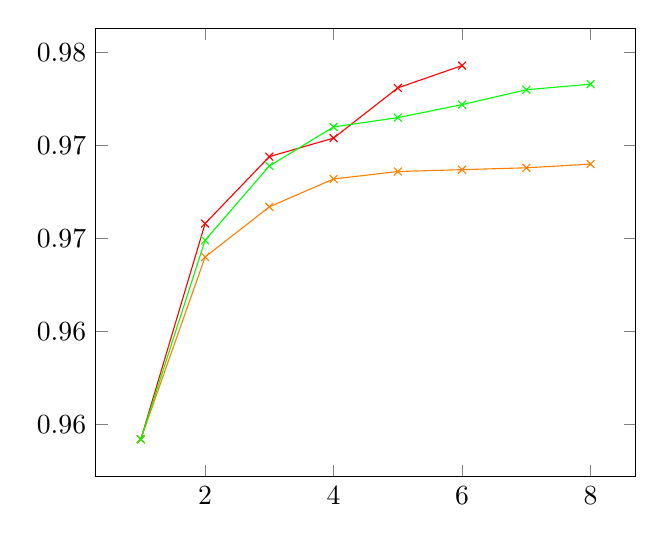
\begin{tikzpicture}
\begin{axis}
    \addplot[color=red,mark=x] coordinates {
        (1.000000 ,  1- 0.045800)
        (2.000000 ,  1- 0.034200)
        (3.000000 ,  1- 0.030600)
        (4.000000 ,  1- 0.029600)
        (5.000000 ,  1- 0.026900)
        (6.000000 ,  1- 0.025700)
    };
    % 0.5 0.969
    \addplot[color=orange,mark=x] coordinates {
        (1.000000  , 1-0.045800)
        (2.000000  , 1-0.036000)
        (3.000000  , 1-0.033300)
        (4.000000  , 1-0.031800)
        (5.000000  , 1-0.031400)
        (6.000000  , 1-0.031300)
        (7.000000  , 1-0.031200)
        (8.000000  , 1-0.031000)
    };
    % 0.75 0.973
    \addplot[color=green,mark=x] coordinates {
        (1.000000,   1-0.045800)
        (2.000000,   1-0.035100)
        (3.000000,   1-0.031100)
        (4.000000,   1-0.029000)
        (5.000000,   1-0.028500)
        (6.000000,   1-0.027800)
        (7.000000,   1-0.027000)
        (8.000000,   1-0.026700)
    };
\end{axis}
\end{tikzpicture}
\end{center}

\section{Końcowy komentarz}

W przeprowadzonych eksperymentach istotym problemem jest wydajność implementacji.
Uczenie sieci bez użycia GPU, w dotatku na 1 wątku. 
Prawdopodobnie implementacja octave (nie ważne na czym skompilowana)
nie korzysta z pełni możliwości jednoski wektorowej procesora przy mnożeniu macierzy.
Z tych powodów uczenie bardzo małego prostego modelu,
dla bardzo małego i prostego zbioru jak MNIST jest bardzo wolne
(około godziny na 1 model zamiast np. 5 minut)
i eksperymentowanie staje się bardziej uciążliwe.

Inną niedogodnością jest wpisywanie ręcznie wzorów na pohodne straty po wagach.
Współcześnie istnieje wiele narzędzi do automatycznego obliczania pochodnej
zadanej funkcji po zadanej zmiennej (np. wagach warstwy) -- w grafowej reprezentacji.

\end{document}
